\chapter{概率论初步}

\section{随机事件与概率}

\subsection{随机事件及其概率}
在一定的条件下,可能发生也可能不发生的事件称为随机事件.

\begin{example}
    掷一枚硬币,“正面向上”这一事件可能发生,也可能不发生,因此,它是一随机事件。
\end{example}

\begin{example}
    对准靶发射一枪,“中靶”这一事件可能发生,也可能不发生,因此,它是一随机事件.
\end{example}

\begin{example}
    将1,2,3这三个数字随便排列,就得一个三位数,“这个三位数大于300”可能发生,也可能不发生,因此,它是一随机事件.
\end{example}


在现实世界中,有许多事件在一定的条件下,可能发生也可能不发生,这些都是随机事件. 通常,我们用大写的英文字母$A,B,C,\ldots$表示随机事件,概率就是反映随机事件出现的可能性大小的一个量;在同一条件下,有些事件发生的可能性比另一些更大些,它们相应的概率也就比另一些的大一些,所以随机事件的概率是客观存在的,问题是如何求出随机事件相应的概率. 为了讨论方便起见,习惯上把“必然事件”与“不可能事件”也看作随机事件。“必然事件”就是在给定条件下必然发生的事件,通常用字母$U$表示. “不可能事件”就是在给定条件下必然不发生的事件,通常用字母$V$表示.在例3.1中,“正面向上或反面向上”就是一个必然事件,“正面和反面都向上”就是一个不可能事件;在例3.3中,“三位数小于400”是一个必然事件,“三位数小于110”就是一个不可能事件.

为了讨论反映随机事件的可能性的大小的量——概率。我们进一步考察“投掷一枚硬币”、“从50只三级管中任抽一只检查”这样一类随机现象。例如,投掷一枚硬币,共有“出现正面”和“出现反面”两种试验结果,通常总认为硬币是“均匀的”,所以出现这两种结果的可能性是相同的。类似地,从50只三级管中任抽一只,共有50种不同的结果,而且只要检查员事先不带主观偏见,抽到任何一只的可能性都相同. 今后,我们称每一试验结果为基本事件,在具体问题中,弄清楚所有基本事件是十分重要的事,首先要注意到不同的基本事件是不能同时发生的;其次要注意到事件总是由若干个基本事件组成. 某一事件所包含的基本事件发生了,就说该事件发生了.

从这两个例子可以看到,这一类随机现象有两个共同的特征:
\begin{enumerate}[(1)]
    \item 有限性:上面每次试验只可能有有限种不同的结果,即有限个基本事件;
    \item 等可能性:由于其自然对称性,出现每一基本事件的可能性是相同的.
\end{enumerate}

这是一类最简单但却是常见的随机现象,我们称它为古典概率模型(简称古典概型),如何来描述这类事件的可能性的大小呢?例如我们问:“50只三级管中有2只次品,从
中任抽一只,抽得次品的可能性有多大?”人们常常用“次品率”来描述这种可能性,这时,次品数(2)和全产品数(50)之比为$2/50=4\%$.我们就说这批三级管的次品是4\%.对于上面的分母和分子,我们也可以这样来看:50是抽一只检查(看作一次试验)时所有可能的基本事件数,2是“抽一只检查得次品”这一事件所包含的基本事件数.

因此对于古典概型,如果试验的基本事件总数为$n$,随机事件$A$所包含的基本事件数为$m$,我们就用数$m/n$来描述每次试验中事件$A$出现的可能性的大小,称它为事件$A$的概率,记作$\Pr(A)$. 即我们定义
\[\Pr(A)=\frac{m}{n}\]

于是对“投掷一枚硬币出现正面”这一随机事件中,由于试验的基本事件总数为2,而“出现正面”只包含其中一个基本事件,所以它的概率等于1/2.对于这样定义的概率显然有

\begin{blk}
    {性质1} \[\Pr(U)=1,\qquad \Pr(V)=0\]
\end{blk}

因为必然事件$U$包含了所有基本事件,所以$\Pr(U)=\frac{n}{n}=1$,而不可能事件$V$不含任何基本事件,所以$\Pr(V)=\frac{0}{n}=0$.

\begin{blk}
 { 性质2}\[0\le \Pr(A)\le 1\]  
\end{blk}

因为事件$A$所含基本事件数$m$满足不等式$0\le m\le n$,所以$0\le \Pr(A)\le 1$.

要算出基本事件总数及A所包含的基本事件数,“排列”、“组合”常常是十分有用的工具.

\begin{example}
    $1,2,3,5,6$六个数字中任取两数,试计算它们都是偶数的概率.
\end{example}

\begin{solution}
    六个数字中任取两个,共有$\comb{2}{6}=15$种不同的取法,这就是全体基本事件,即$n=15$. 而事件$A$:“任取两数都是偶数”则要从$2,4,6$三个偶数中取两个,也就是说事件$A$包含$\comb{2}{3}=3$个基本事件,因此它的概率
\[Pr(A)=\frac{\comb{2}{3}}{\comb{2}{6}}=\frac{3}{15}=\frac{1}{5}\]
\end{solution}


\begin{example}
    在一批零件中有$n$个一等品,$m$个三等品,逐个进行检查. 若已查明前$k\;(k<n)$个均为一等品,求第$k+1$次检查时仍得一等品的概率.
\end{example}

\begin{solution}
    由于已查明前$k$个均为一等品,所求第$k+1$次检查基本事件总数为$n+m-k$,“得一等品”这一事件包含的基本事件数为$n-k$. 因此所求的概率
    \[P=\frac{n-k}{n+m-k}\]
\end{solution}


\begin{example}
    一部四卷文集,按任志次序放到书架上,问各卷自左至右或自右至左的卷号恰为1, 2, 3, 4的顺序的概率是多少?
\end{example}

\begin{solution}
    一部四卷文集,在书架上可有$\perm{4}{4}=4!=24$种不同的排列方法,其中自左至右或自右至左卷号恰为1, 2, 3, 4的顺序的共有2种.因此所求的概率
    \[P=\frac{2}{24}=\frac{1}{12}\]
\end{solution}

\begin{example}
    某停车场有12个位置列成一行.求有8个位置停了车而空着的四个位置连在一起的概率.
\end{example}

\begin{solution}
12个位置中占去8个,共有$\comb{8}{12}$种方法,把四个接连的空位看作一个位置,发生四个接连的位置空着的情形相当于这个假想的位置插入8个停车位置中间或者它们的两端,共有9种不同方法,因此所求的概率为
\[P=\frac{9}{\comb{8}{12}}=\frac{1}{55}\]
\end{solution}

\begin{example}
    鱼池中共有鱼$N$条,从中捕得$t$条,加了标志后立即放回池中,经过一段时间后,再从池中抽出$n$条鱼,问其中有$s$条标志鱼的概率是多少?
\end{example}

\begin{solution}
    从$N$条鱼中捕得$n$条,共有$\comb{n}{N}$种可能结果,它就是基本事件总数. 在捕得的$n$条鱼中恰有$s$条标志鱼,它们是从$t$条标志鱼中捕得的,这种捕法共有$\comb{s}{t}$种. 而对于这样的每一种捕法,其余的$n-s$条未加标志的鱼是从$N-t$条鱼中捕得的,共有$\comb{n-s}{N-t}$种捕法. 因此“捕得$n$条鱼,其中$s$条是标志鱼”的捕法共有$\comb{s}{t}\comb{n-s}{N-t}$种,所求概率
\[P_s(N)=\frac{\comb{s}{t}\comb{n-s}{N-t}}{\comb{n}{N}}\]
\end{solution}

\begin{example}
    某小组有成员3人,每人在某星期7天中参加劳动一天,如果劳动日期可随机安排,求3人在不同的3天参加劳动的概率.
\end{example}

\begin{solution}
    对于某一组员(甲)来说,他可以安排在7天中的任何一天参加劳动,即有7种安排方法,而对于甲的任何一种安排另一组员(乙)又可有7种安排法,因此甲乙两人共有$7^2$种不同的安排法。类似地,对于$7^2$种的任何一种安排,第三名组员(丙)又可有7种安排法.因此所有可能的安排法——总的基本事件数等于$7^3$,而3人安排在7天中的不同的3天有${\rm A}^3_7$种不同的方法,所以要求的概率为
\[P=\frac{{\rm A}^3_7}{7^3}=\frac{30}{49}\]
\end{solution}

上述例3.9颇具典型性,$N$个人在$n$天中的任意安排法相当于把$N$个球随机地放入$n$个盒子里去的方法,共有$N^n$种. 这一类问题称为盒子模型.

\begin{ex}
\begin{enumerate}
    \item 指出下列事物是必然事件,不可能事件,还是随机事件.
\begin{enumerate}[(1)]
\item 如果$a$,$b$都是实数,那么$a+b=b+a$;
\item 从一副扑克牌中任意抽取两张,得到“黑桃”;
\item 某电话总机在一分钟内接到20次呼唤.
\end{enumerate}
\item 某班有50位同学而其中女同学占15名.今碰到这个班的同学,正好碰到一个男同学的概率是多少?正好碰到一个女同学的概率是多少?这两个概率之间有什么关系?为什么?
\item 盒中有100个铁钉,其中有90个是合格的,而10个是坏的,从中任意抽取10个,问其中没有一个为坏的概率是多少?
\item 设袋中有8个球,其中5个白球3个红球,从中任意抽取4个,问恰好抽到3个白球的概率是多少?
\item 两袋分别盛着写有0, 1, 2, 3, 4, 5六个数字的六张卡片,从每袋中各取一张,求所得两数之和等于6的概率.现在有人给出下述两种不同解答:

解1:两数之和共有$0,1,2,\ldots,10$十一种不同结果,因此,所求的概率为$1/11$.

解2:从每袋中各任取一张卡片,共有$6^2$种取法,其中和数为6的情形有5种;
\[(1,5);\quad (2,4);\quad (3,3);\quad (4,2);\quad (5,1)\]
因此所求的概率为$5/36$.

试问哪一种解法正确?为什么?
\item 号码锁上有六个拨盘,每个拨盘上有0—9共10个数字,当这6个拨盘上的数字组成某一个6位数时(第一位可以是0),锁才能打开。如果不知道锁的号码,一次就把锁打开的概率是多少?
\item 设有50张考签,分别加以标号$1,2,\ldots,50$,一学生任意抽一张进行考试,求抽到前10号考签的概率?
\item 一批产品共有100件,其中有次品5件,从中任取10件,求所取10件中至多有2件是次品的概率。
\item 袋中装有$n$个白球和$m$个黑球,从中任取$a+b$个,求所取的球恰含$a$个白球和$b$个黑球的概率?
\end{enumerate}
\end{ex}

\subsection{等可能性事件的概率}
在古典概型里,我们曾规定了$\Pr(A)=m/n$,这是在等可能性的大前提下得出的,这种类型在我们计算事件发生的
概率时是常常碰到的,也是较为重要的,为着重视这种类型,我们再深入研究这类问题.

\begin{example}
    一个均匀材料造的正方体玩具,各个面上分别标以数字$1,2,3,4,5,6$,这种玩具叫骰子,
\begin{enumerate}[(1)]
\item 将骰子抛掷一次,朝上的一面出现奇数的概率是多少?
\item 抛掷2次,朝上的一面的数字之和为7的概率是多少?
\end{enumerate}
\end{example}

\begin{solution}
\begin{enumerate}[(1)]
\item 朝上的一面可为$1,2,3,4,5,6$等六种之一,且每种可能性相等,朝上一面出现奇数,可为$1,3,5$等三种之一,且每种可能性相等,设所问的事件概率为$\Pr(A)$,则$\Pr(A)=\frac{3}{6}=\frac{1}{2}$
\item 抛掷二次,每次朝上一面可有六种情况,两次则共有$6\x6=36$种情况,朝上一面的数字之和为7,则有第一次是1,第二次是6,第一次是6,第二次是1等两种情况。
2与5;3与4,又各有两种,总共有6种,故概率$P=\frac{6}{36}=\frac{1}{6}$.
\end{enumerate}
\end{solution}

\begin{example}
    一次掷三枚骰子,得3点,4点,5点,10点的概率各是多少?
\end{example}

\begin{solution}
\begin{enumerate}[(1)]
    \item 得3点的概率,掷三颗骰子共有216种情况,而得3点只有三颗都为1时的一种,故掷得3点的概率为$\frac{1}{216}$;
    \item 掷三颗骰子共有216种情况,而得4点有$2,1,1$; $1,2,1$; $1,1,2$等三种情况,故掷得4点的概率为$\frac{3}{216}=\frac{1}{72}$;
\item 掷三颗骰子共有216种情况,而得5点有$1,1,3$; $1,3,1$; $3,1,1$; $2,2,1$; $2,1,2$; $1,2,2$,即$\comb{1}{3}+\comb{2}{3}=6$种,故掷得5点的概率为$\frac{6}{216}=\frac{1}{36}$;
\item 掷三颗骰子共有216种情况,而得10点有$1,3,6$; $1,4,5$; $2,2,6$; $2,3,5$; $2,4,4$; $3,3,4$等六种
情况.而$1,3,6$;$1,4,5$;$2,3,5$各有$\perm{3}{3}$种排列.$2,2,6$;$2,4,4$;$3,3,4$有$\comb{1}{3}$种组合. 共有$3\perm{3}{3}+3\comb{1}{3}=27$种. 10点的概率为$\frac{27}{216}=\frac{1}{8}$.
\end{enumerate}  

读者试将掷三颗骰子得3点至18点各点数的概率分别求看看各个概率之间有什么关系,各个概率之和又是什么?
\end{solution}

\begin{example}
    袋中装有$a$个白球和$b$个黑球,从中任意地取出$k+1$($k+1\le a+b$)个球,每次取一球,取后不放回,求最后取出的一球是白球的概率?
\end{example}

\begin{solution}
    从$a+b$个球中无放回地接连取出$k+1$个球,一共有
$(a+b)(a+b-1)\cdots(a+b-k-1+1)={\rm A}^{k+1}_{a+b}$种取法。

$A$表“取出的$k+1$个球中最后一球是白球”的事件。最后取出的白球可以是$a$个白球中的任何一个,有$a$种;而其余$k$个可以是余下的$a+b-1$中的任意$k$个,有${\rm P}^k_{a+b-1}$种取法,因此事件$A$共含$a\cdot {\rm P}^k_{a+b-1}$个不同的基本事件,故所求概率为
\[\Pr(A)=\frac{a{\rm P}^{k}_{a+b-1}}{{\rm P}^{k+1}_{a+b}}=\frac{a}{a+b}\]

从上式可以看出,$\Pr(A)$的值与$k$无关,它说明了无论在哪个序号上,取出白球的概率总是相同的。
\end{solution}

\begin{example}
    有$n$个可辨的球,随机地放入$N\; (N\ge n)$个盒中,每一个盒可以放任意多个球,试求:
\begin{enumerate}
\item 指定的$n$个盒中各有一球的概率?
\item 某$n$个盒中各恰有一球的概率?
\item 某指定的一个盒中恰有$m$($m\le n$)个球的概率?
\end{enumerate}
\end{example}

\begin{solution}
    设球以同样的可能性落入$N$个盒中的每一个,$N$个盒中落一个球一共有$N$种方法,$n$个球可以有$N^n$种方法,这就是总的基本事件数.
\begin{enumerate}
\item 以$A$表“指定的$n$个盒中各有一球”的事件.今固定某$n$个盒,第一个球可以落入这$n$个盒中的任何一个,有$n$种方法,第二个球可落在余下的$n-1$个盒中的任何一个,有$n-1$种方法,……,第$n$个球落在最后的一个盒,只能有一种方法,因此事件$A$共含有$n!$个不同的基本事件,故所求概率为
\[\Pr(A)= \frac{n!}{N^n} \]
\item 以$B$表“某$n$个盒中各恰有一球”的事件.因为$n$个盒可从$N$个盒中任意选取,共有$\comb{n}{N}$种选法. 选出这$n$个盒后再按问题1知事件$B$共含$\comb{n}{N}n!$个不同的基本事件数,故所求概率为
\[\Pr(B)=\frac{\comb{n}{N}n!}{N^n}\]
\item 
以$C$表“某指定的一个盒中恰有$m$个球”的事件,因为$m$个球可从$n$个球中任意选出,共有$\comb{m}{n}$种选法,其余$m$个球可以任意落入其余的$N-1$个盒中,共有$(N-1)^{n-m}$种落法,因此事件$C$共含$\comb{m}{n}(N-1)^{n-m}$个不同的基本事件,故所求概率为
\[\Pr(C)=\frac{\comb{m}{n}(N-1)^{n-m}}{N^n}\]
\end{enumerate}
\end{solution}

\begin{ex}
\begin{enumerate}
\item 有人说,先后抛掷两枚硬币,只有“两枚都是正面”,“两枚都是反面”,“一枚正面,一枚反面”这3种结果,因此,“两枚都出现正面”这一事件的概率是1/3,这种说法错在哪里?
\item 有100张已编号的卡片(从1号到100号),从中任取1张,计算:
\begin{enumerate}[(1)]
    \item 卡片号是偶数的概率;    \item 卡片号是3的倍数的概率.
\end{enumerate}
\item 掷骰子一枚
\begin{enumerate}[(1)]
\item 掷一次,出现奇数的概率是多少?出现偶数的概率是多少?
\item 抛掷2次,得数字之和为8的概率是多少?
\end{enumerate}
\item 在7张数的卡片中,有4张正数卡片和3张负数卡片.从中任取2张作乘法练习,其积为正数的概率是多少?其积为负数的概率是多少?
\item 某种产品90件,其中甲等品40件,乙等品30件,丙等品20件,在运送这些产品的路上损坏了3件,如果每件产品被
损坏的可能性相同,计算这三等产品中恰好各损坏一件的概率.
\item 在80件产品中,有50件一等品,20件二等品,10件三等品.从中任取3件,计算
\begin{enumerate}[(1)]
\item 三件都是一等品的概率;    \item 2件是一等品,1件是二等品的概率;    \item 一等品,二等品三等品各有一件的概率.
\end{enumerate}

\item 六本不同的书,三本封面是红色,三本封面是兰色,将它们任意排列在书架的同一层上,问六本书封面颜色相间的概率是多少?
\item 在一副扑克牌(52张)中,有“黑桃,红心,梅花,方块”这四种花色的牌各13张,从中任取4张,这4张牌的花色相同的概率是多少?这四张牌的花色各不相同的概率是多少?
\item 有五根细木棍,它们的长度分别为1, 3, 5, 7, 9厘米,从中任取三根,它们能搭成一个三角形的概率是多少?
\end{enumerate}
\end{ex}

\subsection{互斥事件与加法定理}
在10个乒乓球中,有7个一等品,2个二等品,1个三等品,我们把从中任取一个,取出一等品叫做事件$A$,取得二等品叫做事件$B$,取出三等品叫做事件$C$. 我们看到,如果取出的乒乓球是一等品,即事件$A$发生,那么事件$B$就不发生. 如果取出的是二等品,那么事件$B$发生,那么事件$A$就不发生,也就是说,事件$A$、$B$不可能同时发生. 这种不可能同时发生的两个事件叫做互斥事件. 同理,事件$B$,$C$是互斥事件,事件$A$,$C$是互斥事件. 换句话说,事件$A$,$B$,$C$中,任何两个都是互斥事件。这时我们说事件$A$,$B$,$C$彼此互斥,一般地,如果事件$A_1,A_2,\ldots,A_n$中任何两个都是互斥事件,那么就说事件$A_1,A_2,\ldots,A_n$彼此互斥.

在上面的问题里,因为是任取一个,共有10种等可能的取法,其中得到一等品,二等品,三等品的取法分别有7种,
2种,1种,因此,$\Pr(A)=\frac{7}{10}$, $\Pr(B)=\frac{2}{10}$, $\Pr(C)=\frac{1}{10}$.

现在问:“任取一个乒乓球,取出一等品或二等品”这一事件的概率是多少?这一事件,我们记作“$A+B$”. 因为不论取出一等品还是二等品,都表示这个事件,发生而得到一等品或二等品的取法共有$7+2$种,所以取出一等品或二等品的概率:
\[\Pr(A+B)=\frac{7+2}{10}\]

由$\frac{7+2}{10}=\frac{7}{10}+\frac{2}{10}$,我们看到
\[\Pr(A+B)=\Pr(A)+\Pr(B)\]
它告诉我们:如果事件$A$,$B$互斥,那么事件“$A+B$”发生(即$A,B$中有一个发生)的概率,等于事件$A$,$B$分别发生的概率的和.

一般地,如果事件$A_1,A_2,\ldots,A_n$彼此互斥,那么事件“$A_1+A_2+\cdots+A_n$”发生(即$A_1,A_2,\ldots,A_n$中有一个事件发生,也叫和事件)的概率,等于这$n$个事件分别发生的概率的和,即
\[\Pr(A_1+A_2+\cdots+A_n)=\Pr(A_1)+\Pr(A_2)+\cdots+\Pr(A_n)\]
这叫做互斥事件的加法定理,也就是说互斥事件的和的概率等于各事件概率之和。

\begin{example}
    某地区的年降水量,在10—150毫米范围内的概率是0.12,在15-200毫米范围内的概率是0.25,在20-250毫米范围内的概率是0.16,在25-300毫米范围内的概率是0.14.计算年降水量在10-200毫米范围内的概率与在15-300毫米范围内的概率.
\end{example}

\begin{solution}
    我们把这个地区的年降水量在10-150毫米,15-200毫米,20-250毫米,25-300毫米范围内分别叫做事件$A$,$B$,$C$,$D$. 很明显,这四个事件彼此互斥,根据公式,年降水量在10-200毫米范围内的概率是
\[\Pr(A+B)=\Pr(A)+\Pr(B)=0.12+0.25=0.37\]
年降水量在15-300毫米范围内的概率是
\[\Pr(B+C+D)=\Pr(B)+\Pr(C)+\Pr(D)=0.25+0.16+0.14=0.55\]
\end{solution}


\begin{example}
    在20件产品中,有15件一级品,5件二级品,从中任取3件,其中至少有1件为二级品的概率是多少?
\end{example}

\begin{solution}
    我们把从20件产品中任取3件,其中恰有1件二级品,叫做事件$A_1$;恰有2件二级品,叫做事件$A_2$;3件全是二级品,叫做事件$A_3$,这样,事件$A_1$,$A_2$,$A_3$的概率分别是
\[\begin{split}
    \Pr(A_1)&=\frac{\comb{1}{5}\cdot \comb{2}{15}}{\comb{3}{20}}=\frac{105}{228}\\
    \Pr(A_2)&=\frac{\comb{2}{5}\cdot \comb{1}{15}}{\comb{3}{20}}=\frac{30}{228}\\
    \Pr(A_3)&=\frac{\comb{3}{5}}{\comb{3}{20}}=\frac{2}{228}\\
\end{split}\]

很明显,事件$A_1$,$A_2$,$A_3$彼此互斥,根据公式,3件产品中至少有1件为二级品的概率是
\[\Pr(A_1+A_2+A_3)=\Pr(A_1)+\Pr(A_2)+\Pr(A_3)=\frac{105}{228}+\frac{30}{228}+\frac{2}{228}=\frac{137}{228}\]

从20件产品中任取3件,或者都是一级品,或者不都是一级品(即其中至少有一件是一级品),这两个互斥事件必有一个发生,这种其中必有一个发生的两个互斥事件,叫做对立事件. 一个事件$A$的对立事件通常记作$\overline{A}$,根据对立事件的意义,$A+\overline{A}$是一个必然事件,它的概率等于1.又由于$A$与$\overline{A}$互斥,我们得到
\[\Pr(A)+\Pr(\overline{A})=\Pr(A+\overline{A})=1\]
这就是说,两个对立事件的概率的和等于1.

从上面公式还可得到$\Pr(\overline{A})=1-\Pr(A)$. 
运用这个公式计算事件的概率,有时比较简单.如例3.15还可以这样来解:

从20件产品中任取3件,3件全是一级品(记作事件$A$)的概率:
\[\Pr(A)=\frac{\comb{3}{15}}{\comb{3}{20}}=\frac{91}{228}\]
由于“任取3件,至少有一件为二级品”是事件$A$的对立事件$\overline{A}$,因此,
\[\Pr(\overline{A})=1-\Pr(A)=1-\frac{91}{228}=\frac{137}{228}\]

读者可想想,什么时候用事件的对立事件的概率来计算就比较简单.
\end{solution}

\begin{example}
一个匣子中有红球5个,白球2个,从匣中随便取出两个球,而球的颜色恰好一样的概率是多少?
\end{example}

\begin{solution}
\textbf{解1:} 令$A=$两球颜色一样,$B_1=$两球颜色均为红色,$B_2=$两球颜色均为白色,可见$B_1$和$B_2$互斥,并且$A=B_1+B_2$,因此
\[\Pr(A)=\Pr(B_1)+\Pr(B_2)\]

今从7个球中随便取出两个球,共有$\comb{2}{7}=\frac{7\x 6}{2}=21$种不同的取法,即简单事件总数为21.$B_1$为两球都为红色,即此两球由红球中取得,所以共有$\comb{2}{5}=\frac{5\x4}{2}=10$个简单事件,
因此$\Pr(B_1)=\frac{\comb{2}{5}}{\comb{2}{7}}=\frac{10}{21}$

$B_2$为两球均为白色,即此两球由白球中取得,所以共有
$\comb{2}{2}=1$个简单事件,于是$\Pr(B_2)=\frac{\comb{2}{2}}{\comb{2}{7}}=\frac{1}{21}$,
因此
\[\Pr(A)=\Pr(B_1)+\Pr(B_2)=\frac{10}{21}+\frac{1}{21}=\frac{11}{21}\]

\textbf{解2:}令$A=$“两球颜色一样”,则$\overline{A}=$“两球颜色不一样”,所以
\[\Pr(\overline{A})=\frac{\comb{1}{5}\cdot \comb{1}{2}}{\comb{2}{7}}=\frac{5\x 2}{21}=\frac{10}{21}\]
因此
\[\Pr(A)=1-\Pr(\overline{A})=1-\frac{10}{21}=\frac{11}{21}\]
\end{solution}

一般地说,如果匣中有$m$个红球,$n$个白球,如果从匣中随便抽取两个球,两球颜色相同的概率$P$可以用完全一样的方法,求得其值为
\[P=\frac{\comb{2}{m}}{\comb{2}{m+n}}+\frac{\comb{2}{n}}{\comb{2}{m+n}}=\frac{m(m-1)+n(n-1)}{(m+n)(m+n-1)}=1-\frac{\comb{1}{m}\cdot \comb{1}{n}}{\comb{2}{m+n}}\]

更一般地,如果匣中有$k$种球,第$i$种球共有$n_i$个,从匣中随便取出两个球,这两个球的颜色是一样的概率是多少呢?这也可用类似的方法求出,读者自己去算一下.

\begin{example}
    从52张扑克牌中随便抽取三张.问:
\begin{itemize}
\item $A=$三张花色相同,
\item $B=$三张是“顺子”(即点数相连),
\item $C=$三张是同花顺子(即花色相同,且点数相连)
\end{itemize}
各自出现的概率是多少?
\end{example}

\begin{solution}
从52张牌中随机抽取三张牌,全部基本事件的总个数是
\[\comb{3}{52}=\frac{52\x 51\x 50}{1\x 2\x 3}=52\x 17\x 25\]
注意到花色有四种,令
\[\begin{split}
    A_1=\text{三张都是梅花},&\qquad 
A_2=\text{三张都是方块}\\
A_3=\text{三张都是红心},&\qquad 
A_4=\text{三张都是黑桃}
\end{split}\]
则$A_1,A_2,A_3,A_4$是互斥事件,且$A=A_1+A_2+A_3+A_4$. 又
\[\begin{split}
    \Pr(A_1)&=\Pr(A_2)=\Pr(A_3)=\Pr(A_4)\\
    &=\frac{\comb{3}{13}}{\comb{3}{52}}=\frac{13\x 12\x 11}{52\x 51\x 50}\\
    &=\frac{11}{17\x 50}=\frac{11}{850}
\end{split} \]
因此,$\Pr(A)=4\Pr(A_1)=\frac{22}{425}$.

三张是顺子,从顺子的点数相连这一要求来看,不计花色,共有“$2,3,4$”,“$3,4,5$”,……“$J,Q,K$”,“$Q,K,A$”这十一种不同的情况,依次用$B_1,B_2,\ldots,B_{11}$来表示它们,于是$B_1,B_2,\ldots,B_{11}$互斥,而且是等概率的,于是
\[\Pr(B)=\Pr(B_1)+\cdots +\Pr(B_{11})=11\Pr(B_1)\]

现在来求$\Pr(B_1)$的值.出现“$2,3,4$”这样的顺子,共有$(\comb{1}{4})^3$这么多种,这是因为这时不考虑花色,同点数的牌每样又有四张,所以出现“$2,3,4$”必须在“2”的四张中取出一张,“3”的四张中取出一张,“4”的四张中取一张,因此,共有$(\comb{1}{4})^3=4^3$这么多种,于是
\[\begin{split}
    \Pr(B_1)&=\frac{4^3}{\comb{3}{52}}=\frac{4^3}{52\x 17\x 25}=\frac{16}{13\x 17\x 25}\\
    \Pr(B)&=\frac{11\x 16}{13\x 17\x 25}=\frac{176}{5525}=\frac{8}{23}\Pr(A)
\end{split}\]
显然$\Pr(B)<\Pr(A)$.

再来计算事件$C$的概率,很明显,从上面的讨论中可以看出来,“$2,3,4$”同花的只可能有四种不同的情形.因此
\[\Pr(C)=\frac{11\x 4}{\comb{3}{52}}=\frac{11}{13\x17\x25} =\frac{1}{6}\Pr(B)\]
显然$\Pr(C)<\Pr(B)$

\end{solution}

\begin{example}
   掷四枚硬币,用“1”表示正面向上,用“0”表示反面向上,于是记$x_i$为第$i$枚硬币的结果,每掷一次,$(x_1,x_2,x_3,x_4)$就表示各枚硬币正、反面的出现情况,例如,
\begin{center}
   (1, 1, 0, 0)就是(正,正,反,反)\\
   (1, 0, 0, 1)就是(正,反,反,正)    
\end{center} 

   求下列各事件的概率:
\[\begin{split}
   A&=\text{恰有两个正面向上}\\
   B&=\text{至少有两个正面向上}\\
   C&=\text{第一枚、第二枚硬币的结果正好相反,第三枚、第四枚硬币的结果正好相反}    
\end{split}\]
\end{example}

\begin{solution}
用$x_1,x_2,x_3,x_4$来表示,就有
\[\begin{split}
   A&=\{x_1+x_2+x_3+x_4=2\}\\
   B&=\{2\le x_1+x_2+x_3+x_4\le 4\}\\
   C&=\{x_1=1-x_2,\; x_3=1-x_4\}    
\end{split}\]

   全部简单事件的个数是一个有重复的排列数,它是$2^4=16$.

\begin{enumerate}[(1)]
    \item   $x_1+x_2+x_3+x_4=2$表示四个数中只有两个是“1",其余两个一定是“0”.而且只要选定了“1”的位置,则“0”的位置也就随之而定了,从四个位置中任选两个,则共有$\comb{2}{4}$种,即6种,因此
   \[\Pr(A)=\frac{6}{16}=\frac{3}{8}\]
   \item $x_1+x_2+x_3+x_4\ge 2$,这一情形可以分成下面三种等式的情形:
\[\begin{split}
    x_1+x_2+x_3+x_4=2&\qquad (\text{有$\comb{2}{4}=6$种情形})\\
    x_1+x_2+x_3+x_4=3&\qquad (\text{有$\comb{3}{4}=4$种情形})\\
    x_1+x_2+x_3+x_4=4&\qquad (\text{有$\comb{4}{4}=1$种情形})\\
\end{split}\]
因此,
\[\Pr(B)=\frac{6+4+1}{16}=\frac{11}{16}\]
\item 此时$x_1=1-x_2$, $x_3=1-x_4$,于是只要看$x_1,x_3$联合起来有多少种不同的情形. 从重复排列的计算公式可以知道$x_1$,$x_3$联合起来共有$2^2=4$种不同情况. 因此,可得
\[\Pr(C)=\frac{4}{16}=\frac{1}{4}\]

\end{enumerate}
   
\end{solution}

\begin{ex}
\begin{enumerate}
    \item 判别下列每对事件是不是互斥事件,如果是,再判别它们是不是对立事件.
从一堆产品中任取2件,其中:
\begin{enumerate}[(1)]
\item 恰有1件次品和恰有2件次品;
\item 有次品和全是次品;
\item 有正品和有次品;
\item 有次品和全是正品.
\end{enumerate}

\item 从一批乒乓球产品中任取一个,如果其重量小于2.45克的概率是0.22,重量不小于2.50克的概率是0.20,那么重量在2.45—2.50克范围内概率是多少?
\item 某射手在一次射击中射中10环,9环,8环的概率分别为0.24, 0.28, 0.19.计算这个射手在一次射击中:
\begin{enumerate}[(1)]
    \item 射中10环或9环的概率;
    \item 不够8环的概率.
\end{enumerate}

\item 一个匣子内有9张票,其号数分别为$1,2,\ldots,9$.从中任取2张,其号数至少有1个为奇数的概率是多少?
\item 在50件产品中有45件合格品,5件次品,从中任取3件,计算其中有次品的概率.
\item 从52张中随便抽取五张.问
\begin{itemize}
\item $A=$五张花色相同;
\item $B=$五张是“顺子”;
\item $C=$五张有花顺子;
\item $D=$五张中有四张点数相同(J作11点,Q作12点,K作13点).
\end{itemize}
$A$,$B$,$C$,$D$各自出现的概率是多少?
\item 掷$n$枚硬币,($n$为偶数)
\begin{itemize}
\item $A=$恰有两个正面向上,
\item $B=$至少有两个正面向上,
\item $C=$第一枚、第二枚硬币的结果正好相反,第三枚、第
四枚的结果正好相反,……第$n-1$枚与第$n$枚的结果正
好相反.
\end{itemize}
求$A$,$B$,$C$各事件的概率.
\item 同时掷三颗骰子,得3点至10点的概率是多少?得11点至18点的概率是多少?
\item 掷三颗骰子,得三颗的点数相同的概率是多少?
\item 从52张扑克中任取五张,问得到三张点数相同,其它两张点数也相同的概率.
\end{enumerate}
\end{ex}

\subsection{事件与集合的对应}
我们现在讨论的一些问题,都离不开基本事件. 所以我们可以把基本事件看作衡量随机事件的“最小单位”,它好象是几何中的“点”,集合中的“元素”.而一切随机事件都是由基本事件组成的,这样,事件之间的各种运算,就和集合之间的各种运算完全对应起来,这样既使我们掌握了事件的运算,还使我们进一步理解了集合运算的意义.

在讨论集合运算时,集合中的一个元素称为一个点,用$a$来表示,则$a$和$\{a\}$是不一样的. 前者是一个点,后者是由$a$这一个点组成的单点集,它是一个集合.

当我们用$E_1,\ldots,E_n$表示基本事件时,它相当于集合中的点,随机事件$A$总是由某些基本事件合起来组成的.如
果把一个基本事件$E_i$也看成是随机事件,那就是指由这个$E_i$组成的集合$\{E_i\}$,这个随机事件$\{E_i\}$相当于一个点组成的单点集. 这一点一定要加以注意,不要一开始就发生混淆.

下面将事件间的运算和事件间的关系的各种定义和集合的运算,以及集合的关系对照着列成一张表,以更进一步看清它们之间的联系,也是为了可以用集合语言来理解概率论.





























由这张对照表,可以由集合的关系式得到事件之间的关
系式,符号的含义和上表相同
\begin{enumerate}
\item $V\subset F\subset U$ (相当于$\emptyset\subset S\subset A$) 

不可能事件$\subset$随机事件$\subset$必然事件
\item 若$F_1\subset F_2$, $F_2\subset F_3$, 则$F_1\subset F_3$
(相当于$S_1\subset S_2,\; S_2\subset S_3$时,必有$S_1\subset S_3$)
\item $F\overline {F}= V$, $F+ \overline {F}= U$ (相当于$S\overline{S} = \emptyset$, $S+ \overline{S} = A$) 

注意:此即$F$与$\overline F$之和必然发生,$F$与$\overline{F}$ 之积是不可能事
件。$\overline{F}$是$F$的逆事件,$F$是$\overline{F}$的逆事件,即彼此互为逆事件。
\item 当$F_1\subset F_2$时,$F_1$中所含的简单事件均为$F_2$中的简单事件,由古典概率公式得
$\Pr\left(F_{1}\right)\le  \Pr\left(F_{2}\right)$
\item 由于$F\overline{F}= V$, $F+ \overline {F}= U$, $F$与$\overline{F}$互斥,从加法定理
得到
$$1=\Pr(U)=\Pr(F)+\Pr(\overline{F})$$
因此,
$\Pr(\overline{F})=1-\Pr\left(F\right)$
\end{enumerate}

\section*{习题3.1}
\begin{enumerate}
\item 设有$n$个房间,分给$n$个不同的人,每个人都以同等可能进入每一房间,而且每间房里的人数没有限制,试求不出现空房的概率?
\item 将$n$个可辨的球投入$N$个盒中,每个球都以同等可能落入每一个盒内,求指定某盒是空的概率.
\item 一批产品共$n$件,其中有$k$件废品,求任意抽出的$m$件产品中恰有$\ell$件废品的概率?
\item 某人有$n$把钥匙,其中只有一把能开他的门,他逐把地取钥匙试开,这试开的手续可能需要$1,2,\ldots,n$次试验,试证明在第$i$次,第$j$次打开锁的概率是一样.
\item 袋中装有10个白球5个黑球,第一次从袋中取出一球(不放回),发现是白球,求第二次从袋中取得白球的概率?并比较两次取得白球概率的大小. 如果第一次取得黑球,求第二次取得白球的概率?
\item 在52张扑克牌中任意取13张,问其中至少有一张是10点的概率是多少?
\item 一盒中有5个白球,7个黑球.
\begin{enumerate}[(1)]
    \item 从中任取一球,问取得是白球和取得是黑球的概率各为多少?
    \item 从中任取两球,问取得都是白球的概率、取得一白一黑的概率各为多少?
\end{enumerate}

\item 箱子所装球的总重量为$N$公斤,而每个球为$n$公斤,其中有$m$个是黑球. 求从箱子中任取一球恰巧是黑球的概率.
\item 一表面为红色的正方体被分割成1000个同样大小的小正方体.试求从中任取一小正方体其两面涂有红色的概率.
\item 从写有$a$,$b$,$c$,$d$,$e$的五张卡片中任取两张,求这两张卡片的字母恰好是按字母顺序相邻排着的概率.
\item 在相应地写有2, 4, 6, 7, 8, 11, 12和13数字的八张卡片中任意取两张,求由所取得的两个数字构成的分数为可约的概率.
\item 从1, 2, 3, 4, 5诸数中任取三数,排成三位数,问如此所得三位数是偶数的概率是多少?
\item 求任意取一整数$N$的:(1)平方;(2)四次方;(3)乘任意一整数后,其尾数为1的概率。
(提示:只需讨论个位数.)
\item 在书架中任意放着10本书,求某给定的三本书放在一起的概率.
\item 4个女孩,3个男孩排成一排,求男女相间的概率.
\item 一个匣子里有90只好的、10只次的螺丝钉.如果从中任意取用10只,恰都是好的螺丝钉的概率是多少?
\item 在一个坛子中放有$n_1$个白球,$n_2$个黑球,逐一全部取出,问第一个和最后一个球都为白球的概率是多少?

\item 求出下述两事件的概率:
\begin{enumerate}[(1)]
    \item 10个人的生日在10个不同的月份;
\item 6个人的生日恰巧在两个月中。(提示:“恰巧在两个月中”不包括“集中在某一个月”的情形. 可先考虑6个人的生日在某指定的两个月里有几种可能.再考虑生日集中在任意两个月里有几种可能.)
\end{enumerate}

\item 电话号码由五个数字组成.每个数字可以是$0,1,2,\ldots,9$中的任意一个数,求电话号码是由完全不相同的数字组成的概率.
\item 从一付扑克(52张)中任取四张,求四张牌的花色各不相同的概率.
\item 为了减少比赛场次,把20个球队分成两组(每组10队)进行比赛,求最强的两队被分在不同组内的概率.
\item 掷三枚骰子,得5点以上(包括5点)的概率是多少!
\item 某人的口袋装有1枚五分的硬币,2枚贰分的硬币以及3枚壹分的硬币,他从中任取3枚,取出的总钱数不少于伍分的概率是多少?
\item 把10个运动队先均分成两组预赛,求最强两队被分在:
\begin{multicols}{2}
\begin{enumerate}[(1)]
\item 不同组内;    \item 同一组内的概率.
\end{enumerate}
\end{multicols}

\item 一座楼房有四个大门,两人住在此楼内,问恰好住在同一大门内的概率是多少?
\item 设在一批有1000件一等品,50件二等品的产品中进行质量检查,如果在该批产品中任意抽查10件,结果全是一等品,问在未被抽查的产品中再任意地连续取两件,至少
有一件是一等品的概率是多少?
\item 用火车运载两个工厂生产的同类产品,其中甲厂30件,乙厂20件,有消息证实,在路途中有两件产品损坏,求损坏的是不同厂的产品的概率.
\end{enumerate}

\section{条件概率与独立事件}
\subsection{条件概率}
若一袋内有7个白球,5个红球,设事件$A=$“取出一个白球”,事件$B=$“取出两个白球”,显然
\[\Pr(A)=\frac{\comb{1}{7}}{\comb{1}{12}}=\frac{7}{12},\qquad \Pr(B)=\frac{\comb{2}{7}}{\comb{2}{12}}=\frac{7}{22}\]

如果我们取出一个白球后,不再放回,那么这时再取出两个白球(注意,实际上是取出了三个白球,但取法是先一个,再两个地取,而不是一起取出)的概率
\[\Pr(B')=\frac{\comb{2}{6}}{\comb{2}{11}}=\frac{3}{11}\]
同样的,如果我们取出两个白球后,不再放回,那么这时再取出一个白球的概率
\[\Pr(A')=\frac{\comb{1}{5}}{\comb{1}{10}}=\frac{1}{2}\]

这个例子告诉我们,我们所计算的某个事件出现的概率是根据另一事件的出现这一事实来确定的.

我们把“出现事件$B$的条件下,出现事件$A$”的概率称为事件$A$关于事件$B$的条件概率,记作$P(A|B)$. 对于上面例子,则
\[\Pr(A')=\Pr(A|B)=\frac{1}{2},\qquad \Pr(B')=\Pr(B|A)=\frac{3}{11}\]

另一方面,考虑事件$AB=$“取出三个白球”,则
\[\begin{split}
    \Pr(AB)=\frac{\comb{3}{7}}{\comb{3}{12}}=\frac{7}{44}&=\frac{7}{22}\x\frac{1}{2}=\Pr(B)\Pr(A|B)\\
    &=\frac{7}{12}\x\frac{3}{11}=\Pr(A)\Pr(A|B)\\
\end{split} \]

就是说$A$与$B$事件同时出现的概率,可以通过$B$出现的概率$\Pr(B)$与$A$关于$B$的条件概率$\Pr(A|B)$来表示.

一般地,对任两个随机事件$A$与$B$,若$\Pr(B)>0$,则有:
\begin{equation}
  \Pr(AB)=\Pr(A|B)\cdot \Pr(B)  \qquad \Pr(AB)=\Pr(B|A)\cdot \Pr(A)\tag{1}
\end{equation}
即
\begin{equation}
    \Pr(A|B)=\frac{\Pr(AB)}{\Pr(B)}\qquad \Pr(B|A)=\frac{\Pr(AB)}{\Pr(A)}\tag{2}
\end{equation}

\begin{proof}
    设基本事件的总数为$e$,其中事件$A$所包含的基本事件有$m$个,事件$B$所包含的基本事件有$n$个,因为我们并没有假定事件$A$和$B$互斥,因此一般都存在着既属于事件$A$,
也属于事件$B$的基本事件,(即事件$A\cdot B$所包含的基本事件)设这样的事件共有$r$个(如图)于是:
\[\Pr(B)=\frac{n}{e},\qquad \Pr(AB)=\frac{r}{e}\]

\begin{center}
    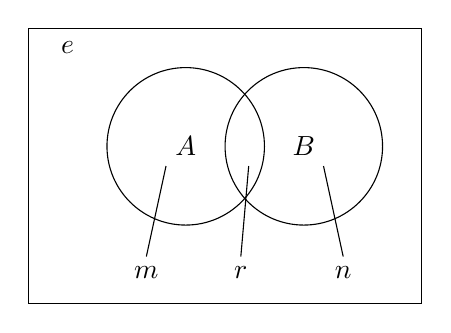
\begin{tikzpicture}
\draw(0,0) rectangle (5,3.5);
\node at (.5,3.25){$e$};
\draw(2,2)node{$A$} circle(1);
\draw(3.5,2)node{$B$} circle(1);
\draw(1.75,1.75)--(1.5,.6)node[below]{$m$};
\draw(3.75,1.75)--(4,.6)node[below]{$n$};
\draw(2.8,1.75)--(2.7,.6)node[below]{$r$};

    \end{tikzpicture}
\end{center}

再看条件概率$\Pr(A|B)$,因为这是在事件$B$发生的条
件下考虑问题的,这时总的基本事件数就是事件$B$所包含的个数$n$,在$B$发生的条件下$A$再发生所包含的基本事件,就必然是属于事件$AB$的$r$个基本事件.

故$\Pr(A|B)=\frac{r}{n}$

这样就有:
\[\Pr(A|B)\cdot\Pr(B)=\frac{r}{n}\cdot \frac{n}{e}=\frac{r}{e}=\Pr(AB)\]
同样可以证明$\Pr(B|A)\cdot\Pr(A)=\Pr(AB)$.
\end{proof}

\begin{example}
    某人提出一个问题,甲先答,答对的概率是0.4;如果答错,由乙答,答对的概率是0.5,求问题由乙解出的概率.
\end{example}

\begin{solution}
“问题由乙解出”相当于“甲答错”($A$)与“乙答对”($B$)两事件一起发生。(即事件$A$,$B$同时发生).

由题意:“甲答错”的概率:$\Pr(A)=1-0.4=0.6$;而“甲答错的条件下乙答对”的概率$\Pr(B|A)=0.5$,
所以“问题由乙解出”的概率:
\[\Pr(AB)=\Pr(B|A)\cdot \Pr(A)=0.5\x0.6=0.3\]
\end{solution}

\begin{example}
    一只袋中有2只白球和3只红球,从袋中取出一只球,然后在第一只不放回的前提下取出第二只球,那么所取出两只球都是红球的概率是多少?
\end{example}

\begin{solution}
    “取出的两只球都是红球”必定是“第一次取得的是红球”($A$),且“第二次取得的是红球”($B$)两事件一起发生(即事件$AB$发生)

    “第一次取置红球”的概率:$\Pr(A)=\frac{3}{5}$,而“第一次取得红球的条件下,第二次取得红球”的概率$\Pr(B|A)=\frac{2}{4}=\frac{1}{2}$,所以“两个球都是红球”的概率:
\[\Pr(AB)=\Pr(B|A)\cdot \Pr(A)=\frac{1}{2}\cdot \frac{3}{5}=\frac{3}{10}\]
\end{solution}

\begin{example}
    某篮球队在己方半场抢得篮板球的概率为0.75而抢得篮板球且反攻投中得分的概率为0.6,问该队已抢得篮板球在手,问这球反攻投中得分的概率有多大?
\end{example}

\begin{solution}
    设事件$A=$“抢得篮板球”;事件$B=$“反攻投中得分”
按题意:$\Pr(A)=0.75$,“抢得篮板球且反攻投中得分”的概率(即积事件$A\cdot B$的概率):$\Pr(AB)=0.6$

所以“抢得篮板球在手,这球反攻投中得分”的概率。
\[\Pr(B|A)=\frac{\Pr(AB)}{\Pr(A)}=\frac{0.6}{0.75}=0.8\]
\end{solution}

\begin{ex}
\begin{enumerate}
    \item 计算在一分钟的区间内进入某邮局的人数的概率如下表:
\begin{center}
\begin{tabular}{cccccc}
\hline
    1分钟内进入的人数&0人&1人&2人&3人&大于3人\\
\hline
概率&0.05&0.15&0.22&0.22&0.36\\
\hline
\end{tabular}
\end{center}    
考虑下述事件:$A=$至少有一个人到达,$B=$至少有二个人到达,$C=$3个顾客到达.

求$\Pr(C|A)$和$\Pr(C|B)$
\item 一个绿骰子和一个红骰子被转动,令$x$表示在红骰子面上出现点子的数目,$y$表示绿骰子面上出现点子的数目.

令:
\begin{multicols}{2}
    $A=$“$x+y>7$的事件”;
    \\
    $B=$“$x+y<6$的事件”;
    \\
    $C=$“$x+y=7$的事件”;\\$D=$“$y=4$的事件”;\\
$E=$“$y=2$的事件”;\\$F=$“$x$或$y$是5”;\\$G=$“$x$和$y$都是5”;\\$H=$“$x+y=10$”
\end{multicols}
求:
\begin{multicols}{3}
 \begin{enumerate}[(1)]
    \item $\Pr(A|D)$
    \item $\Pr(B|E)$
    \item $\Pr(C|D)$
    \item $\Pr(G|F)$
    \item $\Pr(G|H)$
    \item $\Pr(F|H)$
\end{enumerate}   
\end{multicols}
\end{enumerate}
\end{ex}

\subsection{独立事件与乘法定理}
先看下面的问题:“餐桌上摆着10把外形一样的餐刀,其中7把是不锈钢的;3把是镀铬的,记事件$A=$“甲从中任取一把恰为镀铬的”;事件$B=$“乙从中任取一把恰为镀铬的”.

显然,当只有甲单独取用时:$\Pr(A)=\frac{3}{10}$;当只有乙单独取用时:$\Pr(B)=\frac{3}{10}$.

下面再考虑乙先取用的两种情况:
\begin{enumerate}[(1)]
\item 当乙先取用且取得的是镀铬的,用后归还,这相当于返回抽样.

由于这时甲仍是从10把餐刀中取用,其中镀铬的也仍是3把,所以
“乙取得的是镀铬的条件下(用后归还),甲取得的是镀铬的”这一事件的概率:
\[\Pr(A|B)=\frac{3}{10}=\Pr(A)\]
根据同样的分析:$\Pr(B|A)=\frac{3}{10}=\Pr(B)$
\item 当乙先取用且取得是镀铬的,尚未归还甲就取用,这相当于不返回抽样.

这时由于事件$B$的发生,只剩下9把餐刀,其中镀铬的剩下2把,所以
“乙取得的是镀铬的条件下(用后未归还),甲取得的是镀铬的”这一事件的概率:
\[\Pr(A|B)=\frac{2}{9}\ne \Pr(A)\]
根据同样的分析:$\Pr(B|A)=\frac{2}{9}\ne \Pr(B)$
\end{enumerate}

总结上面的分析得出:当乙(甲)的取用不影响甲(乙)的取用,则有下面两等式成立
\[\Pr(A|B)=\Pr(A),\qquad \Pr(B|A)=\Pr(B)\]

当乙(甲)的取用影响到甲(乙)的取用,则:
\[\Pr(A|B)\ne \Pr(A),\qquad \Pr(B|A)\ne \Pr(B)\]

我们定义:如果对于事件$A$和$B$来说,有
\[\Pr(A|B)= \Pr(A),\qquad \Pr(B|A)= \Pr(B)\]
同时成立,那么称事件$A$和事件$B$为相互独立事件,或称事件$A$和$B$相互独立,否则,就是相关的.

对本例,事实上用后归还的话,不管“乙取用为镀铬的”这一事件发生与否,对“甲取用为镀铬的”概率是没有影响的,反之也一样。

因此,通俗地说,事件$A$与$B$相互独立,就是:事件$A$发生与否对事件$B$发生的概率没有影响,同样,事件$B$发生与否对事件$A$发生的概率也没有影响,例如:同时抛掷两枚硬币,记$A=$“第一枚正面向上”,$B=$“第二枚正面向上”;因第一枚是否正面向上对第二枚正面向上的概率没有影响,反之也一样,所以事件$A$与$B$相互独立.

容易看出:当事件$A$和$B$相互独立时,则事件$A$和$\overline{B}$;$\overline{A}$和$B$;$A$和$B$都相互独立的。(读者自己证明)

当事件$A$和$B$相互独立时,上节公式(1)
\[\Pr(AB)=\Pr(A|B)\cdot \Pr(B),\qquad \Pr(AB)=\Pr(B|A)\cdot \Pr(A)\]
变为
\begin{equation}
    \Pr(AB)=\Pr(A)\cdot \Pr(B) \tag{3}
\end{equation}

这就是说:两个相互独立的事件同时发生的概率等于每个事件发生的概率的乘积.

公式(1)和(3)通称为概率的乘法定理。

一般地,若$A_1,A_2,\ldots,A_n$为相互独立事件,则有:
\begin{equation}
    \Pr(A_1\cdot A_2\cdots A_n)=\Pr(A_1)\cdot \Pr(A_2)\cdots \Pr(A_n)\tag{4}
\end{equation}
独立性的概念在概率中是十分重要的,它有广泛的应用. 在实际问题中判断事件是否独立是很重要的.

\begin{example}
    甲乙两人进行一次射击,如果两人射中目标的概率甲为0.6,乙为0.7,计算:
\begin{enumerate}[(1)]
\item 两人都击中目标的概率;
\item 其中恰有一人击中的概率;
\item 至少有一人击中目标的概率。
\end{enumerate}
\end{example}

\begin{solution}
\begin{enumerate}[(1)]
    \item “两人都击中目标”($C$),就是“甲击中目标”($A$),且“乙击中目标”($B$),故$C=A\cdot B$. 事件$A$和$B$显然相互独立,所以
  \[  \Pr(C)=\Pr(A\cdot B)=\Pr(A)\cdot \Pr(B)=0.6\x0.7=0.42\]
    \item “其中恰有一人击中”($D$),就是“甲击中,乙未击中”($A\cdot \overline{B}$)或“甲未击中,乙击中”($\overline{A}\cdot B$),故$D=A\cdot \overline{B}=\overline{A}\cdot B$,显然事件$A\cdot \overline{B}$与$\overline{A}\cdot B$在两人各射击一次时是不可能同时发生的,即事件$A\cdot \overline{B}$与$\overline{A}\cdot B$互斥,所以
\[\begin{split}
    \Pr(D)&=\Pr(A\cdot \overline{B}+\overline{A}\cdot B)=\Pr(A\cdot \overline{B})+\Pr(\overline{A}\cdot B)\\
    &=0.6\x(1-0.7)+(1-0.6)\x 0.7=0.18+0.28=0.46
\end{split}\]
    \item “至少有一人击中”($E$),就是“甲击中,乙未击中”($A\cdot \overline{B}$)或“甲,击中,乙击中”(${A}\cdot B$),或“甲未中乙击中”($\overline{A}\cdot B$),故$E=A\cdot \overline{B}+A\cdot B+\overline{A}\cdot B$,所以
\[\begin{split}
    \Pr(E) &= \Pr(A\cdot \overline{B}+A\cdot B+\overline{A}\cdot B)\\
    &=\Pr(A\cdot \overline{B})+\Pr(A\cdot B)+\Pr(\overline{A}\cdot B)\\
    &=0.6\x0.3+0.6\x0.7+0.4\x0.7\\
&=0.18+0.42+0.28=0.88
\end{split}\]

此小题还可采用下面解法:
“有一个击中”($\overline{E}$),就是“甲未击中”($\overline{A}$)且“乙未击中”($\overline{B}$),故$\overline{E}=\overline{A}\cdot \overline{B}$. 所以:
$$\Pr(\overline{E})=\Pr(\overline{A}\cdot \overline{B})=\Pr(\overline{A})\cdot\Pr(\overline{B})=0.4\x0.3=0.12$$
因此:$\Pr(E)=1-\Pr(\overline{E})=1-0.12=0.88$
\end{enumerate}
\end{solution}

\begin{example}
   假设每枚地-空导弹击中飞机的概率均为0.8,如要有99\%的把握击中来犯敌机,问需几枚导弹同时发射? 
\end{example}


\begin{solution}
设需$n$枚地空-导弹同时发射,
假设事件$A=$“敌机被击中”;“敌机未被击中”($\overline{A}$),就是“第1枚未击中”($\overline{A}_1$),“第2枚未击中”($\overline{A}_2$),……,“第$n$枚未击中”($\overline{A}_n$)同时成立,即:
$\overline{A}_1\cdot \overline{A}_2\cdots \overline{A}_n$,而$\overline{A}_1, \overline{A}_2,\ldots,\overline{A}_n$是彼此独立的事件,因此:
\[\Pr(\overline{A})=\Pr(\overline{A}_1)\cdot \Pr(\overline{A}_2)\cdots\Pr(\overline{A}_n)=(1-0.8)^n=0.2^n\]
要满足击中概率达99\%,即$\Pr(A)=0.99$,故
\[\Pr(\overline{A})=1-\Pr(A)=0.01\]
应满足:$0.2^n=0.01$. 取对数
\[\begin{split}
    n\lg0.2&=\lg0.01\\
n&=\frac{\lg0.01}{\lg0.2}=\frac{-2}{-0.699}\approx 3
\end{split} \]
答:三枚导弹同时发射能以99\%的把握击中来犯敌机.    
\end{solution}

\begin{example}
    一个元件能正常工作的概率$r$称为该元件的可靠性,一组元件组成的系统能正常工作的概率称为系统的可靠性。假设每个使用元件的可靠性都为$r\; (0<r<1)$,且每个元件能否正常工作是相互独立的。试求下面两系统的可靠性,并

\begin{enumerate}[(1)]
    \item 并联通路系统,它由两条$n\; (n\ge 2)$个元件串联成的通路并联而成,如下图
    \item 附加元件系统,它由$n$对并联元件串联而成,如下图
\end{enumerate}
\end{example}

\begin{solution}
    系统(1)有两条通路. 对每条通路来说,必须当每个元件都正常工作时才正常工作,故其可靠性为:$R_c=r^n$

    所以每条通路发生故障的概率为:$1-r^n$.

    系统发生故障,必定是两通路同时发生故障. 故系统发生故障的概率为:$(1-r^n)^2$.

    因此系统(1)的可靠性为:$$R_s=1-(1-r^n)^2=r^n(2-r^n)$$
    所以$R_s>R_c$,即系统在附加了一条通道后,比一条通路增加了可靠性。

    现在考虑系统(2). 从上述讨论易得每对并联元件的可靠性为:$$R'=1-(1-r)^2=r(2-r)$$
    因系统是由各对并联元件串联而成,故其可靠性为:
\[    R_{s'}=(R')^n=r^n(2-r)^n\]
    显然$R_{s'}>R_c$,即用附加元件的方法也能增加系统的可靠性。

两种系统所用的元件一样,其优劣就看可靠性的大小了. 为比较$R_s$与$R_{s'}$的大小,令
$Q_n=\frac{R_{s'}}{R_s}\; (n\ge 2)$,则
\[Q_n=\frac{(2-r)^n}{2-r^n}\]
当$n=2$时:
\[(2-r)^2=2-r^2+2(1-r)^2>2-r^2\]
所以$Q_2>1$

假设当$n=k$时,$Q_k>1$,即$(2-r)^k>2-r^k$,则
\[\begin{split}
 (2-r)^{k+1}>(2-r^k)\cdot (2-r)&=4-2r^k-2r+r^{k+1}\\
&=2-r^{k+1}+2(1-r)(1-r^k)>2-rk+1   
\end{split}\]
即当$n=k+1$时也有$Q_{k+1}>1$

所以对于任意大于等于2的自然数$n$,$Q_n>1$总成立,即$R_{s'}>R_s$,所以系统(2)较系统(1)可靠.
\end{solution}














\section*{习题3.3}
\begin{enumerate}
    \item 生产一种零件,出现次品的概率是0.04,生产这种零件4件,其中恰有1件次品、恰有2件次品、至多有一件次品的概率各是多少?
    \item 某工厂生产中出现次品的概率为0.01,进行重复抽样检查,共取3个样品,求其中次品数等于0, 1, 2, 3的概率.
    \item 设一射手每次中靶的概率为3/5,求四次射击中:
\begin{multicols}{2}
\begin{enumerate}[(1)]
\item 击中一次,    \item 第三次击中,
\item 击中两次,    \item 第二、三两次击中;
\item 至少击中一次的概率。
\end{enumerate}    
\end{multicols}
    \item 有甲乙丙三批罐头,每批100个,其中各有一个是不合格的. 从三批罐头中各抽出一个,计算:
\begin{enumerate}[(1)]
  \item 3个中恰有一个不合格的概率;
\item 3个中至少有一个不合格的概率. 
\end{enumerate}
    \item 某工厂生产过程中出现次品的概率为0.05,每一百个产品为一批,检查产品质量时,在每批中任取一半来检查,如果发现次品不多于1个,则可以认为这批产品是合格的,求一批产品被认为是合格的概率.
\end{enumerate}

\section*{本章内容要点}
一、本章通过大量实例,初步介绍了随机事件的概率及其计算公式.

二、在一定条件下,可能发生也可能不发生的事件,称为随机事件.反映随机事件出现的可能性的大小的一个量,叫做概率.

三、具有有限性、等可能性的特征的随机现象,我们称为古典概型. 如果试验的基本事件总数为$n$,随机事件$A$所包含的事件数为$m$,那么,$A$的概率就定义为$\frac{m}{n}$,记作
\[\Pr(A)=\frac{m}{n}\]
特别地,必然事件$U$的概率为$\Pr(U)=1$; 不可能事件$V$的概率为$\Pr(V)=0$,显然,$0\le \Pr(A)\le 1$.

四、不可能同时发生的两个事件叫 做互斥事件,当$A$,$B$互斥时,
\begin{equation}
    \Pr(A+B)=\Pr(A)+\Pr(B)\tag{*}
\end{equation} 

五、在事件$B$出现的条件下,事件$A$的出现的概率,我们称为$A$关于$B$的条件概率,记作$\Pr(A|B)$. 且有公式
\begin{equation}
   \Pr(A|B)=\frac{\Pr(AB)}{\Pr(B)}\tag{**} 
\end{equation}

六、对于事件$A$,$B$来说,如果有
\[\Pr(A|B)=\Pr(A),\qquad \Pr(B|A)=\Pr(B)\]
同时成立,那么就称事件$A$,$B$为相互独立事件,两个相互
独立的事件同时发生的概率为:
\begin{equation}
    \Pr(A\cdot B)=\Pr(A)\cdot \Pr(B) \tag{***}
\end{equation}

应该注意区别互斥事件、独立事件这两个概念,注意运用公式(*), (***)的前提条件.

七、其中必有一个发生的两个互斥事件,叫做对立事件,当$A$,$B$是对立事件时,有
\[\Pr(A)=1-\Pr(B)\]

八、具有重复试验的结果是相互独立的,而且每次试验的结果只有$A$与$\overline{A}$的特征的随机现象,我们称为重复独立试验概型(又称贝努里概型). 如果事件$A$在一次试验中发生的概率是$P$,那么,它在$n$次独立重复试验中恰好发生$k$次的概率是
\[P_n(k)=\comb{k}{n}P^k(1-P)^{n-k}\]


\section*{复习题三}
\begin{enumerate}
    \item 某种集成电路用到2000小时还能正常工作的概率是94\%,使用到3000小时仍能正常工作的概率是78\%,问已经工作了2000小时的集成电路,能继续工作到3000小时的概率是多少?
    \item 若$M$件产品中包含$m$件废品,今在其中任取两件,求:
\begin{enumerate}[(1)]
\item 已知取出两件中有一件为废品的条件下,另一件也是废品概率;
\item 已知两件中有一件不是废品的条件下,另一件是废品的概率.
\end{enumerate}
    \item 一只瓶含有6个黑球,4个红球和2个绿球,两个球是逐个而不再放回地随机取出,求两个球都是:(1)黑的,(2)红的.(3)绿的,(4)相同的颜色的概率.
    \item 甲袋装有白球3个,黑球5个;乙袋中装有白球4个,黑球6个,现在从甲袋中随意地取出一个球放入乙袋,充分掺混后再从乙袋随意地取出一个球放入甲袋,求这时甲袋中的白球数成下面的情况的概率:
\begin{multicols}{2}
\begin{enumerate}[(1)]
\item 增加,    \item 不变.
\end{enumerate}
\end{multicols}

    \item 在$1,2,\ldots,100$中任取一数,求它既能被2整除又能被5整除的概率,又它能被2整除或能被5整除的概率是多少?
\item 假设总人口中男孩和女孩的比例是1:1,在所有恰有三个孩子的家庭中,求:
\begin{enumerate}[(1)]
\item 一个家庭有两个女孩和一个男孩的概率;
\item 已知最大的孩子是女孩的条件下,一个家庭有两个女孩和一个男孩的概率.
\end{enumerate}

\item 在一个恰有三个孩子的家庭里,若已知:已有(1)一个女孩,(2)一个男孩,求恰有两个女孩的概率是多少?
\item 甲、乙、丙三儿童,甲有红球$a$只,白球$b$只;乙全是红球;丙红、白球都有,三人各拿出1球,其中甲是随机地取出的,丙拿红球或白球的概率都是$\frac{1}{2}$,然后让甲从取出的三个球任意取回一个,求甲的球成下列情况的概率:
\begin{multicols}{3}
\begin{enumerate}[(1)]
\item 红球增加;
\item 红球个数不变;
\item 红球减少.
\end{enumerate}
\end{multicols}

\item 下图是某市街道地图的一部分,一人计划从角落$A$处散步到$B$处,这里往北要走过7条街,往东要过4条街,求:
\begin{enumerate}[(1)]
    \item 从$A$到$B$有几种不同的走法?
    \item 他通过$G$或者$H$的概率是多少?
    \item 他通过标有$G$的拐角处的概率是多少?
    \item 已知他通过$G$或$H$. 求他经过拐角$J$的条件概率.
\end{enumerate}

\item 轰炸机要完成它的使命,必须驾驶员找到了轰炸目标,投弹员又投中了目标,设驾驶员甲和乙找到目标的概率分别为0.9和0.8;又设投弹员丙和丁在驾驶员找到了目标的条件下投中目标的概率分别为0.7和0.6.现在配备两架轰炸机的人员,问甲乙与丙丁应该怎样搭配才能使完成使命有较大的概率?又这个概率比起另一种配合大多少?(只要有一架飞机投中目标即完成使命).
\item 一个工人看管四台机床,如果在一小时内这些机床不需要人去照顾的概率,第一台是0.79,第二台是0.79,第三台是0.80,第四台是0.81,假设各台机床是否需要照顾相互之间没有影响,计算在这个小时内,这四台机床都不需要照顾的概率.
\item 有甲、乙、丙三批罐头,每批分别有100、120、
150个,其中各有3个是不合格的,从三批罐头中各抽出一个,计算:
\begin{enumerate}[(1)]
\item 3个恰有一个合格的概率;
\item 3个中至少有一个不合格的概率。
\end{enumerate}

\item 甲、乙、丙三步枪手射中某目标的概率各为0.7、0.8及0.85;现向该目标各发一弹,问射中3, 2, 1, 0弹的概率各为多少?
\item 两部车床独立地工作,每部车床不需要工人照顾的概率分别为0.9和0.85,求
\begin{enumerate}[(1)]
\item 都不需要照顾的概率;
\item 恰好一台需要照顾的概率;
\item 同时需要照顾的概率.
\end{enumerate}

\item 有一乘客在电车汽车联合站候车,任何一种车都能使他到达目的地. 如果在五分钟内电车到站的概率是$\frac{1}{2}$,汽车到站的概率是$\frac{1}{3}$. 问这个乘客在五分钟内能够登上任何一种车的概率是多少?
\item 甲袋子内有$m$个白球,$n$个黑球,乙袋子内有$n$个白球,$m$个黑球. 从两个袋子内各任意摸出一个,得到一个白球一个黑球的概率是多少?
\item 一箱螺钉共十万只,次品率为0.004,问事件“从中任意抽验一只,是次品;然后又抽验两只,这两只中至少有一只是次品”的概率有多少?
\item 街道交叉口上交通的畅通程度可用任意给定的一秒钟内有一部车子通过的概率P来描述;假定在不同时刻车子的经过是互不影响的,如果一个步行者只能在三秒钟没有车子通过的情形下才能跨过街道,求他恰巧等待0, 1, 2, 3秒钟的概率.
\item 某仪表有$m$个同样的电子管,其中任一个电子管损坏,这个仪表就不能工作,如果在某段时间内每个电子管损坏的概率是$P$,计算在这段时间内,这个仪表不能工作的概率。
\item 在下图所示的开关电路中,开关$A$、$B$、$C$开或关的概率均独立地为$\frac{1}{2}$,求灯点亮的概率.

\item 某种大炮击中目标的概率是0.3,只要以多少门这样的大炮同时射击一次,就可以使击中目标的概率:
\begin{multicols}{2}
\begin{enumerate}[(1)]
\item 超过95\%;    \item 不小于0.99.
\end{enumerate}
\end{multicols}

\item 某售货员在三个柜面上售货,如果在某一小时内柜面需要售货员照顾的概率,第一柜面是0.9,第二柜面为0.8,第三柜面为0.7,假定各个柜面是否需要照顾相互之间不受影响,计算在这个小时内,至少有一个柜面需要售货员的概率.
\item 甲、乙、丙三猎手向同一野猪射击,设甲射中的概率为0.4;乙射中的概率为0.5;丙射中的概率为0.7,若只有一人射中,野猪被击毙的概率为0.2;若其中二人射中,则野猪被击毙的概率为0.6;若三人同时射中,则野猪必定被击毙。求野猪被击毙的概率。
\item 某射手射击一次,击中目标的概率是0.9,他射击了四次。分别写出恰好击中4次,3次,2次,1次,0次的概率,并将它们与$(0.9+0.1)^4$的展开式的各项进行比较,你可得出什么结论?
\item 一次测量中出现正误差和负误差的概率都是$\frac{1}{2}$,在3次测量中,恰好出现2次正误差的概率是多少?恰好出现两次负误差的概率是多少?
\item 一头病牛用某药后被治愈的概率为95\%,计算服用这种药的4头病牛中至少有3头被治愈的概率.
\item 在乒乓球比赛中,甲、乙两人球艺相当,胜负机会相同,试比较下列概率哪一个较大?一方在:
\begin{enumerate}[(1)]
\item 4盘中胜3盘与8盘中胜5盘;
\item 4盘中胜3盘以上与8盘中胜5盘以上;
\item $2n$盘中胜的盘数不多于$n$与$2n$盘中胜$n$盘以上.
\end{enumerate}

\item 每一用户在一小时内向总机拔话的概率等于0.02,该总机有300个分机,试问在一小时内有不少于7个分机向总机拔话的概率是多少?

\item 某一批蚕豆种籽,如果每一粒发芽的概率为90\%,播下5粒种籽,计算:
\begin{enumerate}[(1)]
    \item 其中恰有4粒发芽的概率;
    \item 其中恰有4粒未发芽的概率.
\end{enumerate}

\item 在四次独立试验中,事件$A$至少出现一次的概率为$\frac{80}{81}$,求事件$A$在各次试验中出现的概率.
\item 某小组有10台各为7.5千瓦的机床,如果每台机床的使用情况是互相独立的,且每台机床平均每小时开动12分钟,问全部机床用电超过48千瓦的可能性有多大.
\item 某一学校有730名学生,对每一个人来说,他的生日在某一天的概率设为$\frac{1}{360}$,求:
\begin{enumerate}[(1)]
\item 恰有3名学生的生日为元月1日;
\item 生日在元月1日学生不多于3人;
\item 没有一个学生的生日在元月1日;
\item 至少有一个学生的生日在元月1日的概率.
\end{enumerate}

\item 两个篮球运动员在罚球线投球的命中率分别是0.7与0.6,每人投球3次,计算两人都投进2球的概率.
\item 一个织布工人看管12台布机、在$a$小时内一台布机需要工人照顾的概率等于$\frac{1}{3}$
\begin{enumerate}[(1)]
\item 在$a$小时内,有4台布机需要照顾的概率;
\item 在$a$小时内,需要照顾的布机不多于6台的概率.
\end{enumerate}

\item 在多次试验中,当事件$A$出现不少于3次时,事件B才出现.而事件$A$在每次试验中出现的概率等于0.3,若
\begin{multicols}{2}
    \begin{enumerate}[(1)]
    \item 作了5次试验;
    \item 作了7次试验
\end{enumerate}
\end{multicols}
试求$\Pr(B)$.

\item 一个通讯小组有两套通讯设备,只要其中有一套设备能正常工作,就能进行通讯,每套设备出3个部件组成.只要其中有一个部件出故障,这套设备就不能正常工作,如果在某段时间内每个部件不出故障的概率都是$P$,计算在这段时间内能进行通讯的概率.
\item 甲、乙两个篮球队员各投蓝3次,每次投篮时投中得分的概率各为0.6和0.7.求
\begin{multicols}{2}
\begin{enumerate}[(1)]
    \item 得分相同的概率;
    \item 甲得分比乙多的概率.
\end{enumerate}    
\end{multicols}

\end{enumerate}

